\section{METODOLOGI}
\label{chap:desainimplementasi}

% Ubah bagian-bagian berikut dengan isi dari desain dan implementasi

% Penelitian ini dilaksanakan sesuai \lipsum[1][1-5]

\subsection{Data dan Peralatan / Data dan Alat Bantu / Material}
\label{sec:perlengkapan}


\begin{enumerate}
  \item Dataset
  \par \emph{Dataset} yang digunakan yaitu gambar atau foto yang meliputi gambar personel atau manusia yang menggunaka helm keselamatan kerja dan/atau manusia yang tidak menggunakan helm keselamatan kerja.
  Selama penulisan proposal ini, dataset yang sudah didapatkan yaitu :
  \begin{enumerate}
    \item \emph{Safety helmet detection} oleh andrewmvd
    \par Dataset ini berisi 5000 gambar pekerja konstruksi yang meliputi orang yang menggunakan helm dan yang tidak menggunakan helm keselamatan kerja. Masin - masing gambar sudah diberi label
    \emph{"helmet"} dan \emph{"head"}. Format anotasi label nya berupa fromat PASCAL VOC yang disimpan dalam file .xml.
  \end{enumerate}
  \par Kedepannya akan dilakukan pengumpulan lebih untuk dataset.

  \item Alat Bantu
  \begin{enumerate}
    \item Anaconda
    \par Anaconda sendiri merupakan package distribution yang dibuat khusus untuk data science. Anaconda biasanya digunakan untuk membuat environment baru untuk mengisolasi proyek dan menginstall package untuk keperluan tertentu. Pada penelitian ini akan digunakan untuk membantu penulis dalam mengumpulkan package - package yang diperlukan untuk melakukan proses training dan pengembangan sistem.\cite{pankajmathur_2018}

    \item Python 3.7
    \par Python sendiri adalah bahasa pemrograman high level yang sudah terinterpretasi dan berbasis objek. Struktur data yang sudah ada di dalam python dan penulisan syntax yang sederhana dan mudah dipahami dapat meningkatkan performa pengerjaan. Pada penelitian ini python digunakan karena merupakan bahasa pemrograman yang cocok untuk data science mengingat struktur data di python yang dinamis. Selain itu python juga sudah termasuk saat menginstall Anaconda \cite{python.org}

    \item Visual Studio Code
    \par Visual Studio Code adalah source code editor yang ramah performa dan mudah digunakan untuk segala bentuk keperluan penulisan text sehari - harinya. Visual Code mendukung banyak bahasa pemrograman dan menyediakan fitur addons yang digunakan untuk mendownload package untuk berbagai macam kebutuhan berbeda. Pada penelitian ini Visual Studio Code digunakan untuk menulisa script python yang akan digunakan untuk training, pengembangan sistem, dan keperluan lainyna yang sekiranya dibutuhkan pada penelitian ini dan dapat diselesaikan dengan visual studio code.\cite{microsoft_2021}

    \item Roboflow
    \par Roboflow merupakan \emph{tools} yang membantu developer untuk mengolah segala keperluan untuk melakukan pengembangan di bidang visi komputer. Fasilitas yang ditawarkan oleh Roboflow meliputi : pengorganisasian dataset, 
    pelabelan atau \emph{annotation} , pembagian rasio \emph{train/test}, \emph{preprocessing} yang meliputi re-size ukuran gambar, isolasi objek, grayscale, auto-adjust contrast, tile, dan bahkan sekaligus train. 

  \end{enumerate}


\end{enumerate}



\subsection{Metodologi Penelitian}
\label{metodologipenelitian}

\begin{figure}[ht]
  \centering
  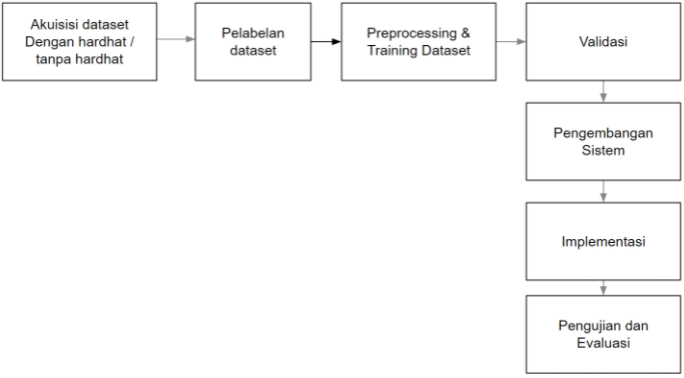
\includegraphics[scale=0.7]{gambar/blockdiagram-helmetdetection.png}
  \caption{Block Diagram Penelitian Deteksi Helm Keselamatan kerja Menggunakan CNN}
  \label{fig:blockdiagramhelmetdetection}  
\end{figure}

\begin{enumerate}
  \item Akuisisi Dataset
  \par Dibutuhkan kumpulan gambar yang digunakan sebagai \emph{dataset} untuk melakukan \emph{training} dengan YOLOv5 untuk menghasilkan bobot yang lalu digunakan untuk melakukan 
  deteksi personel yang menggunakan helm keselamatan kerja dan pengguna yang tidak menggunakan helm keselamatan kerja. Gambar yang akan digunakan perlu meliputi kepala manusia tanpa helm atau
  kepala manusia yang mengenakan helm. Dibutuhkan berbagai variasi untuk tiap ketentuan baik yang mengenakan helm dan yang tidak mengenakan helm dengan harapan akan meningkatkan kemampuan
  prediksi pada saat diimplementasikan pada sistem seperti variasi dari jauh dekat, warna helm, keadaan cuaca atau pencayaannya.
  \par Metode pengumpulan atau akuisisi dataset nya meliputi pencarian atau \emph{browsing} gambar di internet, mengambil dataset yang digunakan oleh penilitian terkait, dan membuat sendiri dari foto
  menggunakan helm keselamatan kerja.

  \item Pelabelan Dataset
  \par Gambar - gambar yang sudah dikumpulkan dan dijadikan dataset perlu diberi pelabelan untuk masing - masing kelas atau label. Pada penelitian ini, label yang dibuat berjumlah 2 yaitu 
  "head" dan "helmet". Pemberian bounding box untuk label \emph{"head"} meliputi dari ujung kepala (rambut) hingga leher dan untuk label \emph{"helmet"} meliputi seluruh bagian helm 
  keselamatan kerja hingga leher. Untuk penelitian ini, helm yang akan dideteksi sebagai label "helm" yaitu helm keselamatan kerja. Anotasi dari pelabelan akan disimpan kedalam format yang diterima oleh YOLOv5 yaitu format PyTorch yang disimpan dalam file .txt dan .yaml untuk \emph{config}.
  Proses pelabelan pada gambar hanya dilakukan pada gambar atau dataset yang belum memiliki pelabelan. Pada dataset yang sudah didapatkan pada penulisan proposal ini, \emph{Safety helmet detection} oleh andrewmvd, sudah memiliki
  pelabelan.
  \par Pelabelan dilakukan menggunakan Roboflow menggunakan fitur \emph{Annotate}. Fitur \emph{Annotate} dari Roboflow memberikan kemudahan ke pengguna dimana pengguna hanya perlu men-drag bounding
  box di area yang akan diberi label dan memilih kelas labelnya. 
  
  \item Preprocessing Dataset
  \par Sebelum dapat digunakan untuk training menggunakan YOLOv5, perlu dilakukan beberapa modifikasi pada dataset yang sudah dikumpulkan. Hal ini dilakukan untuk menyesuaikan konfigurasi 
  yang ditentukan untuk train dan detect. Proses ini meliputi pengaturan rasio jumlah gambar untuk train-test-validation dan re-size gambar.
  \par Pengaturan rasio jumlah gambar untuk train-test-validation dilakukan di Roboflow pada bagian Generate New Version dari dataset yang sudah di upload ke Roboflow. Pada penilitian ini akan dilakukan beberapa percobaan untuk rasio dataset yang akan menghasilkan hasil bobot yang paling bagus.
  \par Pengaturan ukuran gambar akan disesuaikan dengan hardware yang akan digunakan untuk melakukan training menggunakan YOLOv5. Roboflow juga menyediakan fitur \emph{re-size} untuk mengatur ulang
  ukuran gambar.
  \par Setelah melakukan pemrosesan, Roboflow memberikan fitur export yang akan mengoutputkan \emph{command line} untuk download. \emph{Command line} juga disesuaikan untuk versi \emph{pre-processing} yang disimpan
  di Roboflow.

  \item Training Dataset dan Validasi
  \par Untuk melakukan training dataset, digunakan source code yang sudah diberikan dari repository YOLOv5 oleh Glenn Jocher. Dalam melakukan training akan dilakukan beberapa training menggunakan model yang sudah disediakan
  dari YOLOv5 seperti YOLOv5s, YOLOv5m, YOLOv5l, dan YOLOv5x. Bobot yang dihasilkan dari masing - masing training menggunakan model yang berbeda akan dibandingkan \emph{metrics}-nya seperti precision, recall, dan mAP. Format bobot yang dihasilkan
  dari training menggunakan YOLOv5 akan berupa .pt yang nanti bisa dicoba menggunakan source code detect.py yang disediakan juga dari repo YOLOv5.
  Proses training akan dilakukan di hardware milik penulis dan/atau menggunakan \emph{Google Colab}.

  \item Pengembangan Sistem
  \par Perlu dilakukannya pengembangan sistem yang dapat menerima input video real time dari kamera yang lalu dapat melakukan identifikasi penggunaan helm dan tidak yang dimana dilakukan
  dengan menggunakan model yang sudah dibuat. Sistem yang akan menajalankan bobot yang dihasilkan dari training menggunakan YOLOv5 akan dikembangkan dengan asumsi :
  \begin{enumerate}
    \item Jenis input yang akan digunakan untuk deteksi oleh sistem adalah \emph{live-feed} dari kamera.
    \item Kamera yang digunakan untuk mengawasi diletakkan pada checkpoint masuk ke lokasi utama konstruksi dimana outlet listrik umumnya ada pada suatu lokasi konstruksi.
    \item Sistem akan dijalankan pada suatu komputer yang berada di lokasi konstruksi.
    \item Sistem akan memicu atau men-\emph{trigger} suatu mekanisme alarm.
  \end{enumerate} 

  \item Implementasi
  \par Sistem yang selesai dikembangkan akan diimplementasikan untuk melakukan deteksi pada manusia yang menggunakan helm dan yang tidak dengan input dari kamera atau web cam yang mengirimkan input live-feed.
  Implementasinya juga akan dilakukan pada lokasi konstruksi nyata jika memungkinkan.

  \item Pengujian dan Evaluasi
  \par Dari proses implementasi akan dilakukan pengujian keberhasilan dan keefektifan sistem saat dikerahkan pada implementasi dunia nyata.

\end{enumerate}


% % Contoh pembuatan potongan kode
% \begin{lstlisting}[
%   language=C++,
%   caption={Program halo dunia.},
%   label={lst:halodunia}
% ]
% #include <iostream>

% int main() {
%     std::cout << "Halo Dunia!";
%     return 0;
% }
% \end{lstlisting}

% \lipsum[2-3]

% % Contoh input potongan kode dari file
% \lstinputlisting[
%   language=Python,
%   caption={Program perhitungan bilangan prima.},
%   label={lst:bilanganprima}
% ]{program/bilangan-prima.py}

% \lipsum[4]
